\section{Теоретические основы}

Метрическое пространство~---~это пара $ \left( S, d \right) $,
состоящая из множества $S$ и метрики $d \; : \; S \times S \rightarrow \mathbb{R}$,
то есть для любых $x, y, z \in S$ выполняется
\begin{enumerate}
  \item $d \left( x, y \right) \geq 0$;
  \item $d \left( x, y \right) = 0 \Leftrightarrow x = y$~---~аксиома тождества;
  \item $d \left( x, y \right) = d \left( y, x \right) $~---~аксиома симметрии;
  \item $d \left( x, z \right) \leq d \left( x, y \right) + d \left( y, z \right) $ ---
  неравенство треугольника.
\end{enumerate}

Метрическое пространство называется полным,
если любая фундаментальная последовательность его точек имеет предел в этом пространстве.

Множество $X$ точек метрического пространства $ \left( S, d \right) $ называется компактным,
если из любого его открытого покрытия можно выделить конечное число множеств,
которые тоже покрывают множество $X$.

Метрическое пространство $S$ называется сепарабельным,
если для любого $x \in S$ и любого $ \varepsilon > 0$ имеется такой элемент $x_s \in S$,
что $d \left( x, x_s \right) \leq \varepsilon $.

\section{Хаусдорфова мера}

Классическая процедура оценки площади плоской фигуры
заключается в аппроксимации множества $S$ маленькими кубиками, объёмы которых суммируются.
Хаусдорф же заменяет квадраты шарами.

Если $S$ является поверхностью,
то её площадь можно оценить складывая площади $ \pi \rho^2$ каждого шара.
В более общем виде вместо $ \pi \rho^2$ используется пробная функция $h \left( \rho \right) $.
В таком случае можно сказать, что мера конечного покрытия множества $S$
шарами радиуса $ \rho_m$ равна $ \sum \limits_{m \in M} h \left( \rho_m \right) $,
где $M$~---~множество индексов.
Для более экономного покрытия рассматривается покрытие шарами, радиус которых меньше $ \rho $,
и образуется точная нижняя грань
\begin{equation}\label{eq:inf}
  \inf \limits_{ \rho_m < \rho } \sum \limits_{m \in M} h \left( \rho_m \right).
\end{equation}

При $ \rho \to 0$ условие на радиусы шаров становится слишком жёстким,
и выражение \ref{eq:inf} возрастает.
У него есть предел
\begin{equation*}
  \lim \limits_{ \rho \to 0}
  \inf \limits_{ \rho_m < \rho } \sum \limits_{m \in M} h \left( \rho_m \right).
\end{equation*}
Он определяет $h$-меру множества $S$ \cite{mandelbrot}.

Пример такой меры --- логарифмическая $h$-мера при
\begin{equation*}
  h \left( \rho \right) =
  \frac{1}{ln \left| \rho \right| }.
\end{equation*}
Если же $h \left( \rho \right) = \gamma \left( d \right) \rho^2$, где введена функция,
соответствующая протяжённости шара единичного радиуса
\begin{equation*}
  \gamma \left( d \right) =
  \frac{\left[ \Gamma \left( \frac{1}{2} \right) \right]^d}{ \Gamma \left( 1 + \frac{d}{2} \right) },
\end{equation*}
то $h$-мера называется $d$-мерной.

\section{Расстояние Хаусдорфа}

Расстояние Хаусдорфа определяется на множестве
всех непустых компактных подмножеств пространства $ \mathbb{R}^n$.

Пусть $E$ и $F$~---~непустые компактные подмножества $ \mathbb{R}^n$.
Расстояние Хаусдорфа между $E$ и $F$ определяется как
\begin{equation}\label{eq:hausdorff:distance}
  H \left( E, F \right) =
  \min \left\{ \varepsilon > 0 \; | \; E \subset F + \varepsilon, \, F = E + \varepsilon \right\},
\end{equation}
где $E + \varepsilon $~---~объединение замкнутых шаров
с центром в точке $x$ радиуса $ \varepsilon $
\begin{equation*}
  E + \varepsilon =
  \bigcup \limits_{x \in E} \left\{ \overline{B}_{ \varepsilon } \left( x \right) \right\}.
\end{equation*}

\subsection{Пример}

Найдём расстояние Хаусдорфа между двумя эллипсами \ref{fig:hausdorff:example} \cite{crownover}
\begin{gather*}
  E \, : \, \frac{x^2}{4} + 4y^2 = 1, \, \\
  F \, : \, 4 \left( x - 2 \right)^2 + \frac{y^2}{4} = 1.
\end{gather*}

\begin{figure}
  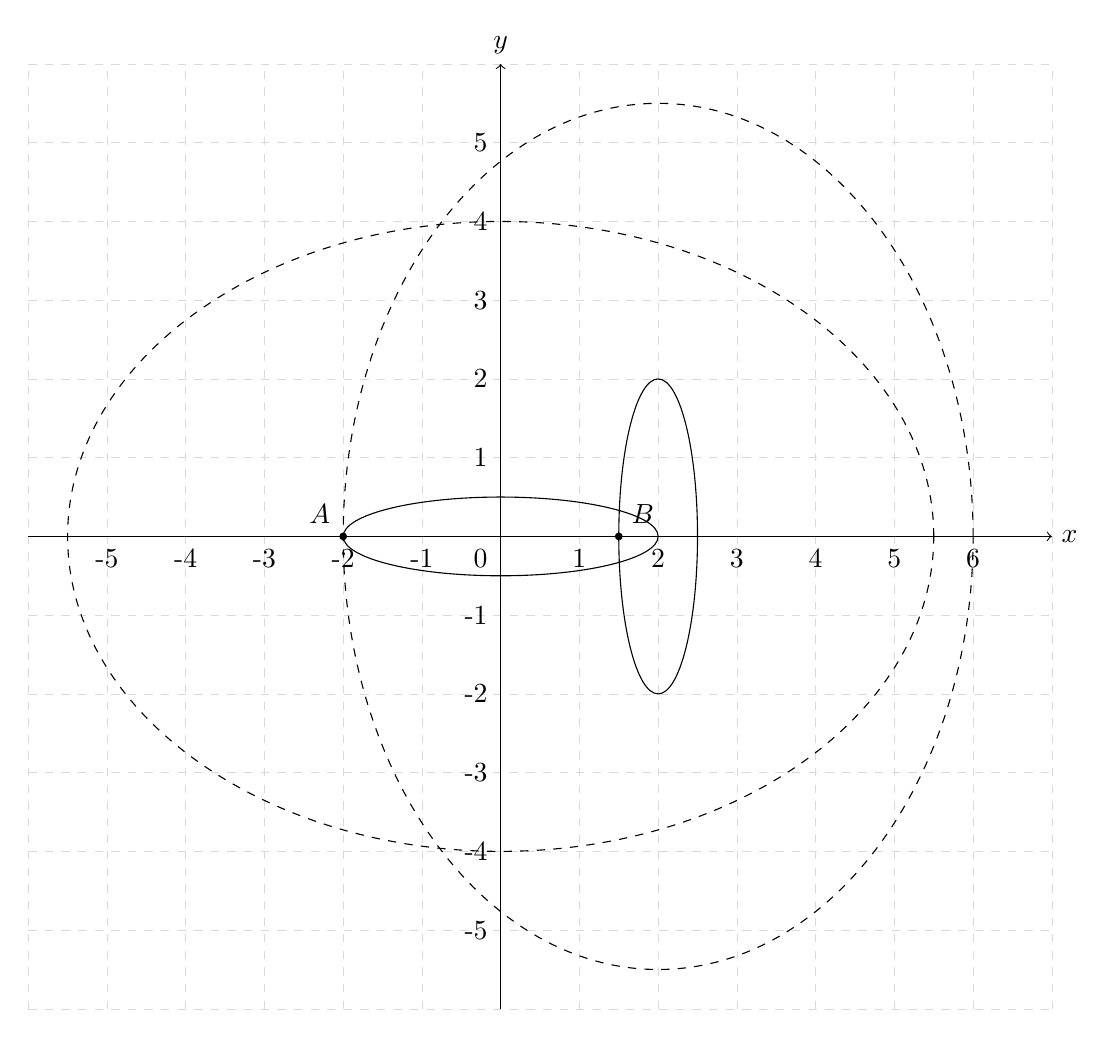
\begin{tikzpicture}
    \draw[help lines, color=gray!30, dashed] (-6,-6) grid (7,6);
    \draw[->] (-6,0)--(7,0) node[right]{$x$};
    \draw[->] (0,-6)--(0,6) node[above]{$y$};
    \node[inner sep=1pt,label=below left:{0}] at (0,0) {};
    \foreach \i in {-5,...,-1,1,2,3,4,5,6}
    {
      \node[inner sep=1pt,label=below:{\i}] at (\i,0) {};
    }
    \foreach \i in {-5,...,-1,1,2,3,4,5}
    {
      \node[inner sep=1pt,label=left:{\i}] at (0,\i) {};
    }
    \draw (0,0) ellipse (2 and 0.5);
    \draw (2,0) ellipse (0.5 and 2);
    \draw[dashed] (0,0) ellipse (5.5 and 4);
    \draw[dashed] (2,0) ellipse (4 and 5.5);
    \node[circle,inner sep=1pt,fill=black,label=above left:{$A$}] at (-2,0) {};
    \node[circle,inner sep=1pt,fill=black,label=above right:{$B$}] at (1.5,0) {};
  \end{tikzpicture}
  \caption{Эллипсы, между которыми ищем расстояние Хаусдорфа}
  \label{fig:hausdorff:example}
\end{figure}

Пунктиром нарисованы эллипсы $E + \varepsilon $ и $F + \varepsilon $ такие,
чтобы выполнялось \ref{eq:hausdorff:distance}.
Таким образом $ \varepsilon $ в данном случае~---~это расстояние между точками $A$ и $B$,
которое равно $ \varepsilon = 1.5 - \left( -2 \right) = 3.5$.
Поэтому $H \left( E, D \right) = 3.5$.
